\chapter{Background}
\section{Computer Vision in Robotics} Computer vision is a broad field that includes methods for acquiring, processing, analyzing and understanding images and, in general, high-dimensional data from the real world in order to produce numerical or symbolic information, e.g., in the forms of decisions \cite{1}.

Proper vision is the utmost importance for the function of any vision based autonomous robot. Areas of artificial intelligence deal with autonomous planning or deliberation for robotic systems to navigate through an environment. A detailed understanding of these environments is required to navigate through them. High-level information about the environment could be provided by a computer vision system that is acting as a vision sensor.

In this thesis, we will focus on the hand gesture recognition using computer vision techniques for a humanoid robot named as NAO, as shown in the figure \ref{fig:nao}. NAO is an autonomous, programmable humanoid robot developed by Aldebaran Robotics. The NAO Academics Edition was developed for universities and laboratories for research and education purposes. Table \ref{tb:nao} shows the specification of NAO according to Aldebaran Robotics.

\subsection{NAO Vision} Two identical video cameras are located in the forehead of NAO. They provide up to 1280x960 resolution at 30 frames per second. NAO contains a set of algorithms for detecting and recognizing faces and shapes.

\subsection{Extending NAO} 
3D cameras such as Microsoft Kinect and Asus Xtion are used not only for gaming but also for analyzing 3D data, including algorithms for feature selection, scene analysis, motion tracking, skeletal tracking and gesture recognition \cite{12}. 

3D model based gesture recognition needs 3D data. Hence we attempt to use Asus Xtion as an external camera that will be mounted on the head of NAO as shown in the figure \ref{fig:xtion}. Computational limitations of NAO hinders us to build an effective real time gesture recognition. Therefore, we propose to use an off-board computer to process the sensor data from NAO, execute the gesture recognition algorithm and finally command NAO to do an appropriate action.

\begin{table}
	[h] \centering \caption{NAO V5 hardware and software specification } \label{tb:nao} 
	\begin{tabular}
		{|l|l|} \hline Height & 58 centimetres (23 in) \\
		\hline Weight & 4.3 kilograms (9.5 lb) \\
		\hline Battery autonomy & 60 minutes (active use), 90 minutes (normal use) \\
		\hline Degrees of freedom & 21 to 25 \\
		\hline CPU & Intel Atom @ 1.6 GHz \\
		\hline Built-in OS & Linux \\
		\hline SDK compatibility & Windows, Mac OS, Linux \\
		\hline Programming languages & C++, Python, Java, MATLAB, Urbi, C, .Net \\
		\hline Vision & 2 x HD 1280x960 cameras \\
		\hline Connectivity & Ethernet, Wi-Fi \\
		\hline \multirow{6}{*}{Sensors} & 4 x directional microphones \\
		& 1 x sonar rangefinder \\
		& 2 x IR emitters and receivers \\
		& 1 x inertial board \\
		& 9 x tactile sensors \\
		& 8 x pressure sensors \\
		\hline 
	\end{tabular}
\end{table}

\begin{figure}
	\centering
	\begin{minipage}{.5\textwidth}
		\centering
		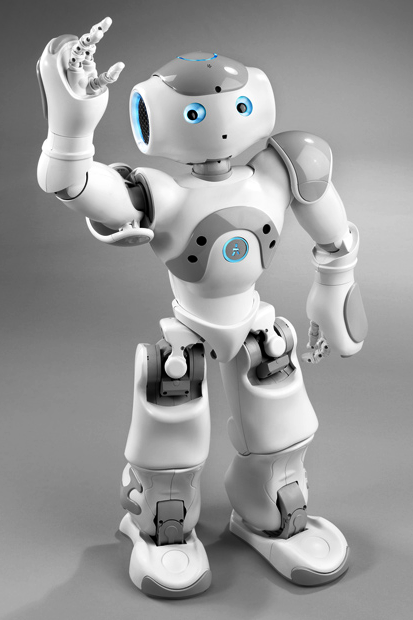
\includegraphics[height=7cm]{figures/nao.png} 
		\captionof{figure}{NAO}
		\label{fig:nao}
	\end{minipage}%
	\begin{minipage}{.5\textwidth}
		\centering
		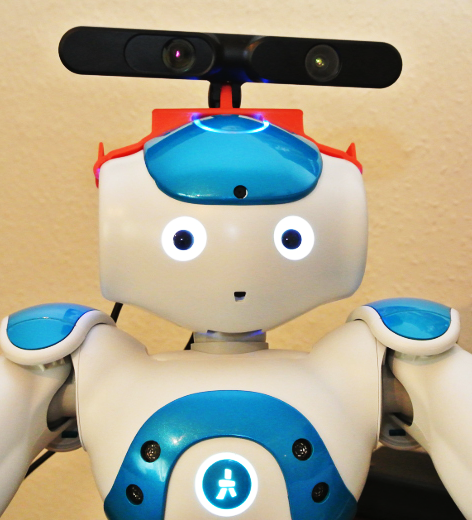
\includegraphics[height=7cm]{figures/nao-xtion.png} 
		\captionof{figure}{Asus Xtion mounted on NAO }
		\label{fig:xtion}
	\end{minipage}
\end{figure}


\section{Gesture Recognition} 


Human hand gestures are a means of non-verbal interaction among people. They range from simple actions of using our hand to point at, to the more complex ones that express our feelings and allow us to communicate with others. To exploit the use of gestures in HRI, it is necessary to provide the means by which they can be interpreted by robots. The HRI interpretation of gestures requires that dynamic and/or static configurations of the human hand, arm and even other parts of the human body, be measurable by the machine \cite{6}. 

Initial attempts to recognize hand gestures resulted in electro-mechanical devices that directly measure hand and/or arm joint angles and spatial position using sensors \cite{3}. Glove-based gestural interfaces require the user to wear such a complex device that hinders the ease and naturalness with which the user can interact with the computer controlled environment. 

Even though such hand gloves are used in highly specialized domain such as simulation of medical surgery or even in the real surgery, the everyday user will be certainly deterred by such sophisticated interfacing devices. As an active result of the motivated research in HRI, computer vision based techniques were innovated to augment the naturalness of interaction.

\subsection{Gesture Modeling} 
Figure \ref{fig:ges:model} shows various types of modeling techniques used for Gesture modeling \cite{3}. Selection of an appropriate gesture modeling depends primarily on the intended application. For an application that needs just hand gesture to go up and down or left and light, a very simple model may be sufficient. However, if the purpose is a natural-like interaction, a model has to be sophisticated enough to interpret all the possible gesture. The following section discusses various gesture modeling techniques which are being used by the existing hand gesture recognition applications. 

\begin{figure}
	[h] \centering 
	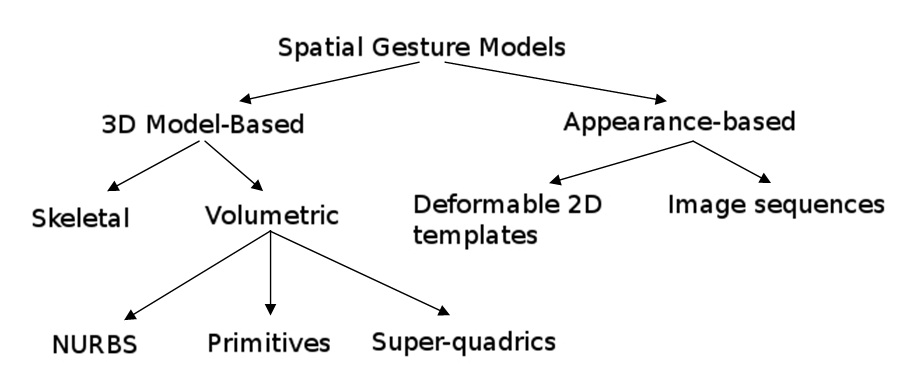
\includegraphics[height=5cm]{figures/ges-model.png} 
	\caption{Classification of gesture modeling \cite{10}.}
	\label{fig:ges:model} 
\end{figure}

Appearance based models don't use the spatial representation of the body, because they derive the parameters directly from the images or videos using a template database. 

3D hand based model approach uses volumetric or skeletal models, or even a combination of  both. Volumetric approaches have been heavily used in computer animation industry and for computer vision purposes. The models are generally created of complicated 3D surfaces. The drawback of this method is that is very computational intensive. 

Instead of using intensive processing of the 3D hand models and dealing with a lot of parameters, one can just use a simplified version that analyses the joint angle parameters along with segment length. This is known as a skeletal representation of the body, where a virtual skeleton of the person is computed and parts of the body are mapped to certain segments \cite{4}. The analysis here is done using the position and orientation of these segments and the relation between each one of them.

In this thesis, we focus on Skeletal based modeling algorithms which are faster because the detection program has to focus only on the significant parts of the body. Moreover, it allows to do pattern matching against a template database. 

\subsection{Gestural Taxonomy }
Several alternative taxonomies have been suggested that deal with psychological aspects of gestures \cite{3}. All hand/arm movements are first classified into two major classes as shown in the figure \ref{fig:ges:tax}.

\begin{figure}
	[h] \centering 
	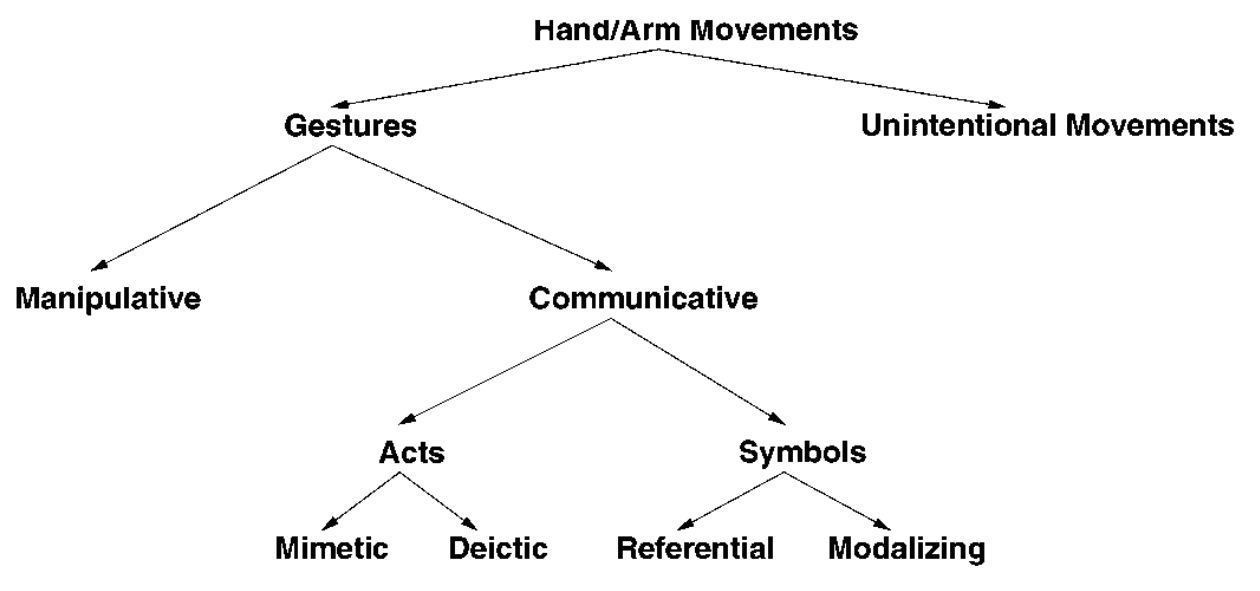
\includegraphics[width=12cm]{figures/ges-tax.png} 
	\caption{Classification of gestures \cite{3}.}
	\label{fig:ges:tax} 
\end{figure}

Manipulative gestures are the ones used to act on objects. For example, moving a chair from one location to another. Manipulative gestures in the context of HRI are mainly developed for medical surgery. Communicative gestures, on the other hand, have purely communicational purpose. In a natural environment they are usually accompanied by speech or spoken as a sign language. In HRI context these gesture are one of the commonly used gestures, since they can often be represented by static as well as dynamic hand postures.

In this thesis, we focus on communicative gestures in the form of symbols. They symbolize some referential action. For instance, circular motion of hand may be referred as an alphabet "O" or as an object such as wheel or as a command to turn in a circular motion .


\subsection{Gesture Recognition}
The task of gesture recognition shares certain similarities with other recognition tasks, such as speech recognition and biometrics. Though alternatives such as Dynamic Programming (DP) matching algorithms have been attempted, the most successful solutions involves feature-based statistical learning algorithm, usually Hidden Markov Models \cite{5}. 

In this thesis, we have chosen a machine learning technique based on hidden Markov model to recognize gestures. HMM is a statistical model in which the system being modeled is assumed to be a Markov process with unobserved (hidden) states. In simpler Markov models, the state is directly visible to the observer and therefore the state transition probabilities are the only parameters. In a hidden Markov model, the state is not directly visible, but output dependent on the state is visible.

\section{Software and Libraries}
\subsection{OpenNI 2}
\subsection{NiTE 2}
\subsection{UDP}
\subsection{Websocket}
\subsection{WebGL ThreeJS}
